% Editable native annotations around unchanged verified IDE photographs.
\par
\begin{figure}[htbp]
  \centering
  \newsavebox{\MARScrcFailuremissingregistersBox}
  \sbox{\MARScrcFailuremissingregistersBox}{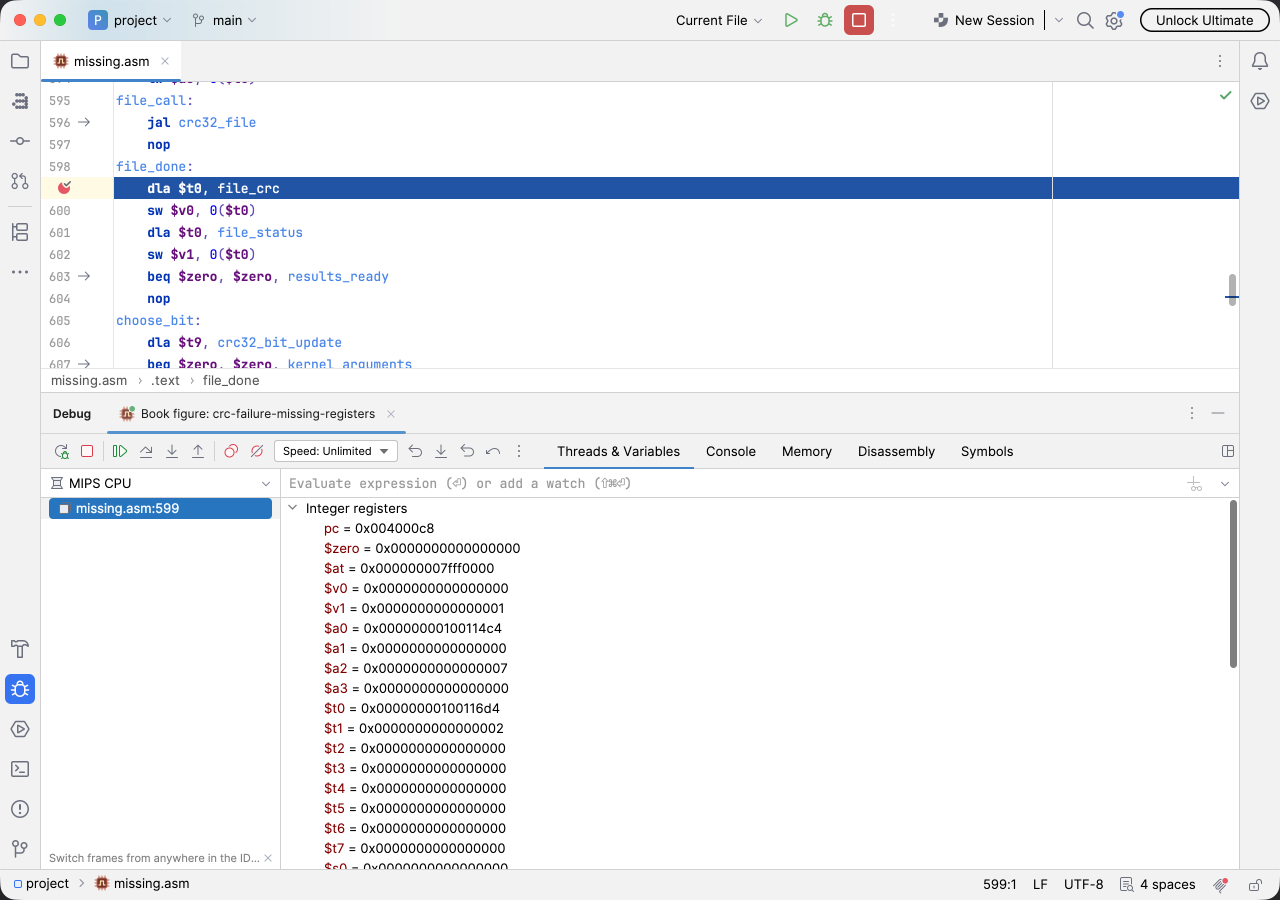
\includegraphics[artifact]{packages/024-crc32/captures/f04/missing-registers.png}}
  \newsavebox{\MARScrcFailurereaderrorregistersBox}
  \sbox{\MARScrcFailurereaderrorregistersBox}{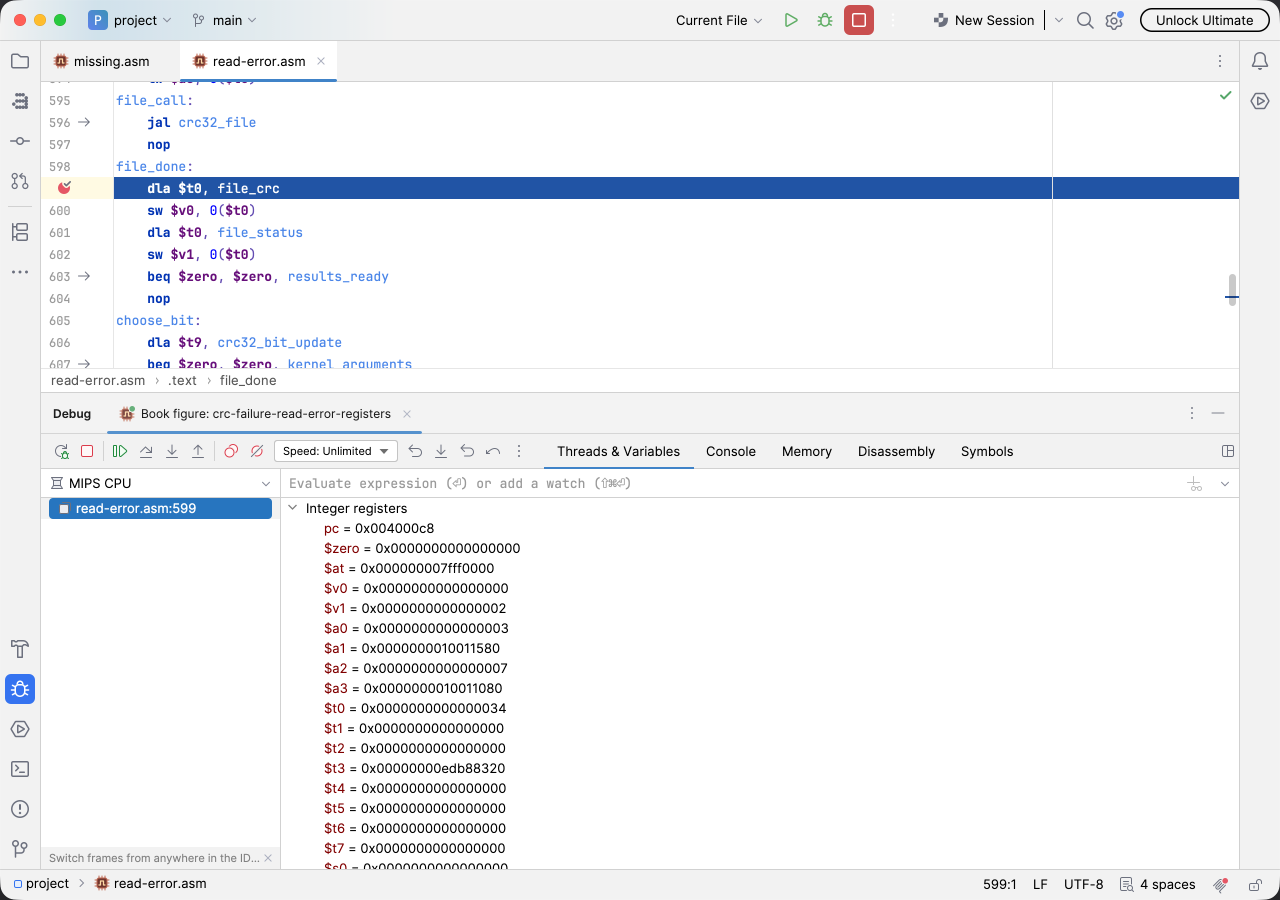
\includegraphics[artifact]{packages/024-crc32/captures/f04/read-error-registers.png}}
  \newsavebox{\MARScrcFailuremissingscratchBox}
  \sbox{\MARScrcFailuremissingscratchBox}{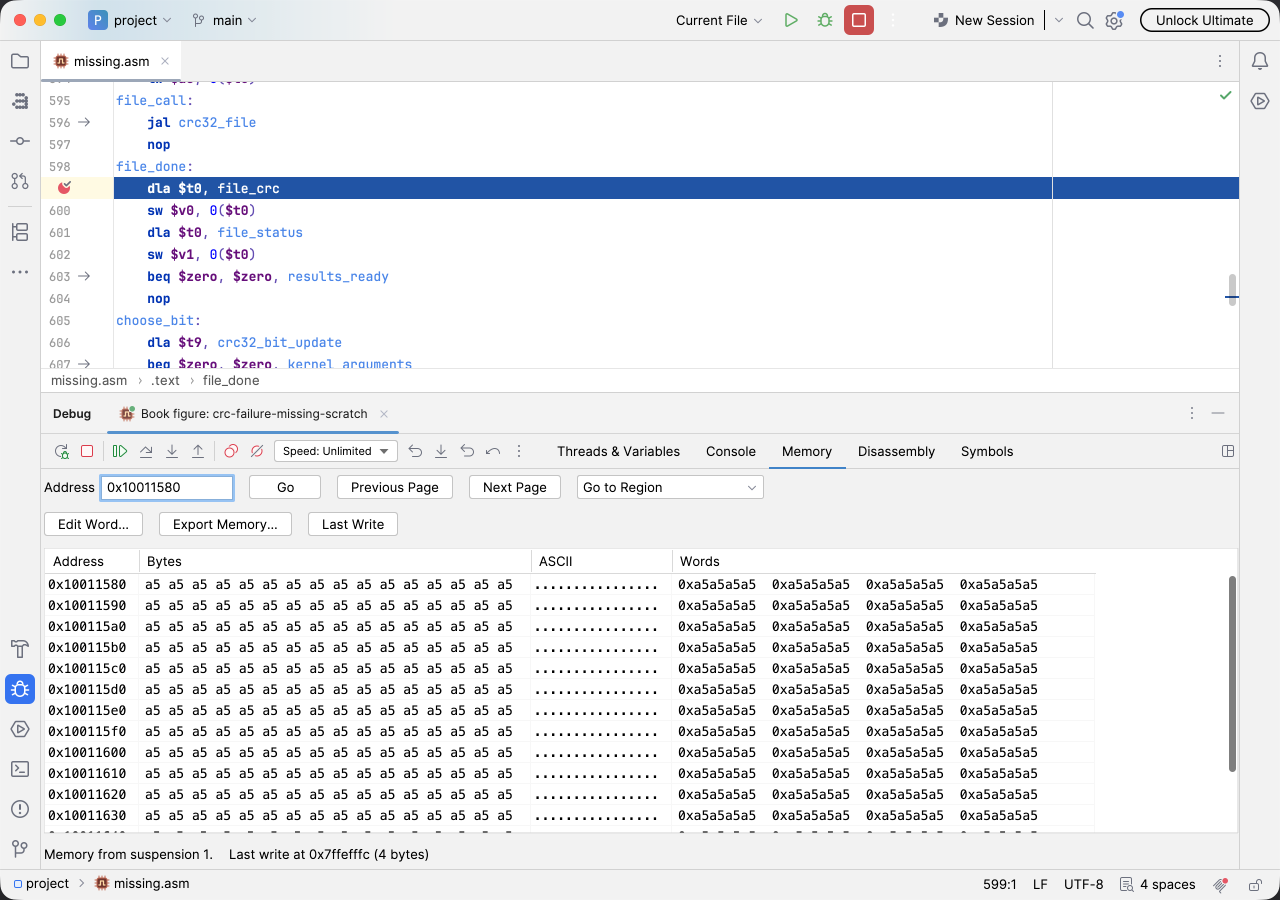
\includegraphics[artifact]{packages/024-crc32/captures/f04/missing-scratch.png}}
  \newsavebox{\MARScrcFailurereaderrorscratchBox}
  \sbox{\MARScrcFailurereaderrorscratchBox}{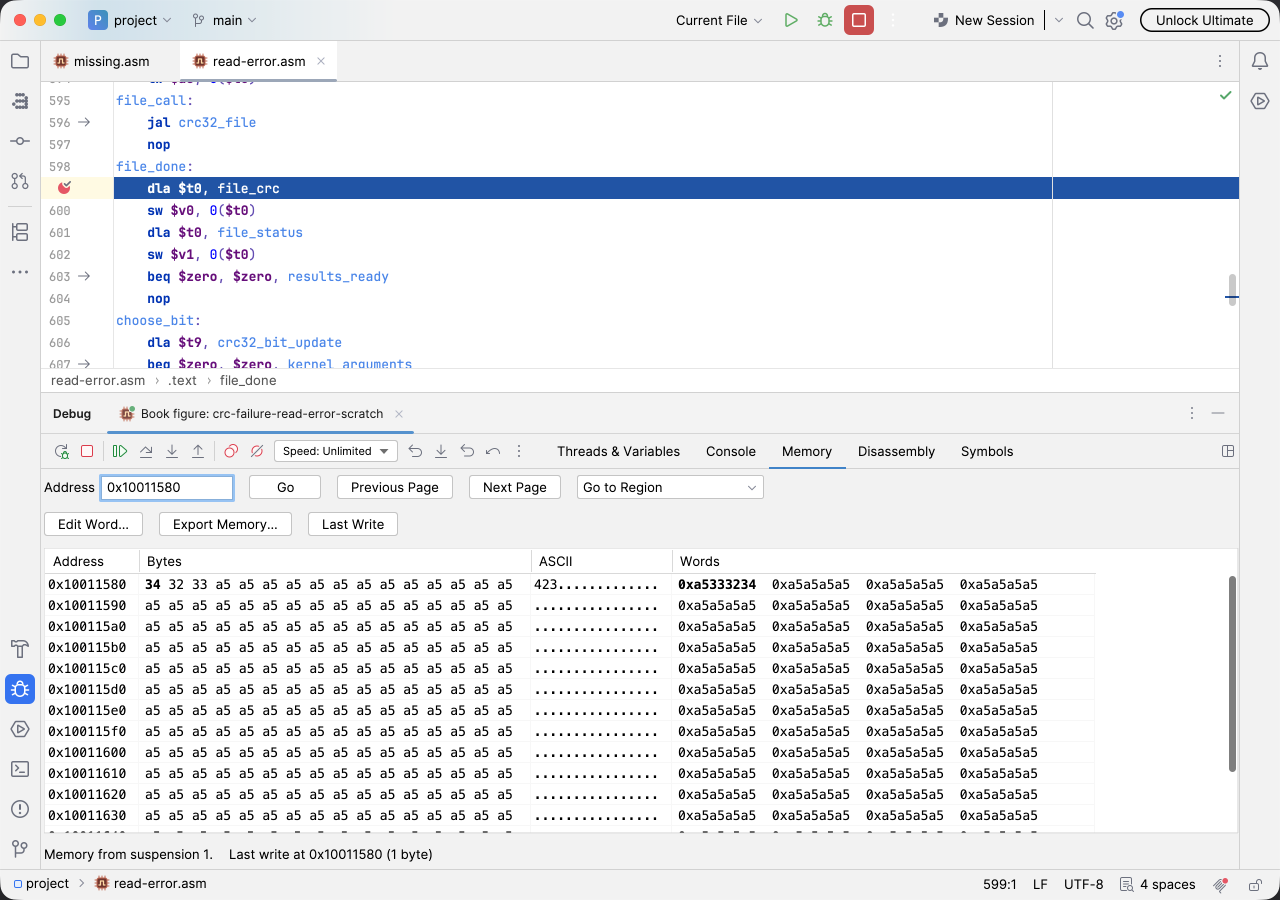
\includegraphics[artifact]{packages/024-crc32/captures/f04/read-error-scratch.png}}
  \newsavebox{\MARScrcFailurereaderrorcontrolBox}
  \sbox{\MARScrcFailurereaderrorcontrolBox}{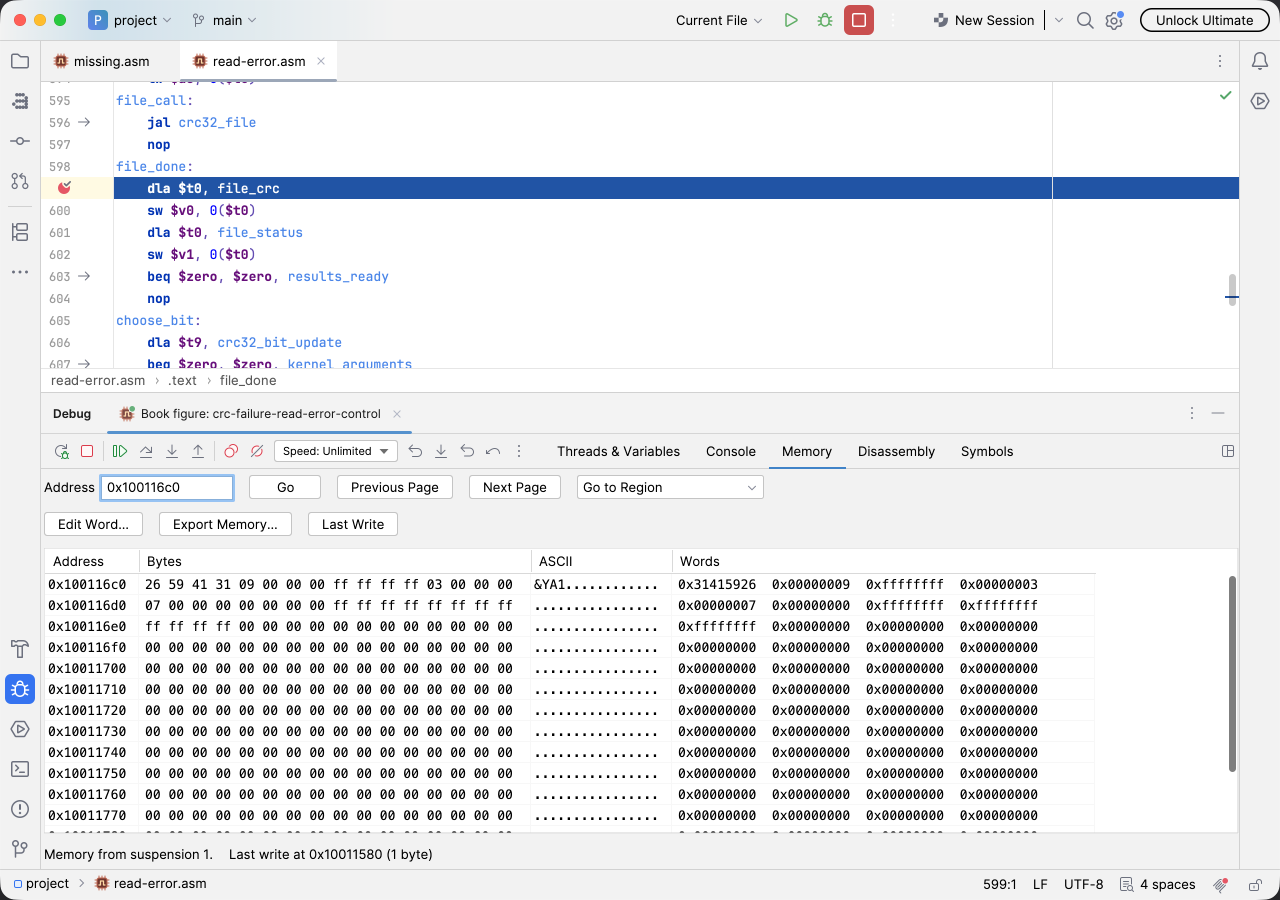
\includegraphics[artifact]{packages/024-crc32/captures/f04/read-error-control.png}}
  \edef\MARScrcFailuresourceLeft{\the\dimexpr0.036718750\wd\MARScrcFailurereaderrorregistersBox\relax}
  \edef\MARScrcFailuresourceBottom{\the\dimexpr0.774444444\ht\MARScrcFailurereaderrorregistersBox\relax}
  \edef\MARScrcFailuresourceRight{\the\dimexpr0.713281250\wd\MARScrcFailurereaderrorregistersBox\relax}
  \edef\MARScrcFailuresourceTop{\the\dimexpr0.170000000\ht\MARScrcFailurereaderrorregistersBox\relax}
  \edef\MARScrcFailuremissingLeft{\the\dimexpr0.246093750\wd\MARScrcFailuremissingregistersBox\relax}
  \edef\MARScrcFailuremissingBottom{\the\dimexpr0.312222222\ht\MARScrcFailuremissingregistersBox\relax}
  \edef\MARScrcFailuremissingRight{\the\dimexpr0.553906250\wd\MARScrcFailuremissingregistersBox\relax}
  \edef\MARScrcFailuremissingTop{\the\dimexpr0.640000000\ht\MARScrcFailuremissingregistersBox\relax}
  \edef\MARScrcFailurereaderrorLeft{\the\dimexpr0.246093750\wd\MARScrcFailurereaderrorregistersBox\relax}
  \edef\MARScrcFailurereaderrorBottom{\the\dimexpr0.312222222\ht\MARScrcFailurereaderrorregistersBox\relax}
  \edef\MARScrcFailurereaderrorRight{\the\dimexpr0.553906250\wd\MARScrcFailurereaderrorregistersBox\relax}
  \edef\MARScrcFailurereaderrorTop{\the\dimexpr0.640000000\ht\MARScrcFailurereaderrorregistersBox\relax}
  \edef\MARScrcFailuremissingscratchLeft{\the\dimexpr0.034375000\wd\MARScrcFailuremissingscratchBox\relax}
  \edef\MARScrcFailuremissingscratchBottom{\the\dimexpr0.334444444\ht\MARScrcFailuremissingscratchBox\relax}
  \edef\MARScrcFailuremissingscratchRight{\the\dimexpr0.584375000\wd\MARScrcFailuremissingscratchBox\relax}
  \edef\MARScrcFailuremissingscratchTop{\the\dimexpr0.608888889\ht\MARScrcFailuremissingscratchBox\relax}
  \edef\MARScrcFailureerrorscratchLeft{\the\dimexpr0.034375000\wd\MARScrcFailurereaderrorscratchBox\relax}
  \edef\MARScrcFailureerrorscratchBottom{\the\dimexpr0.334444444\ht\MARScrcFailurereaderrorscratchBox\relax}
  \edef\MARScrcFailureerrorscratchRight{\the\dimexpr0.584375000\wd\MARScrcFailurereaderrorscratchBox\relax}
  \edef\MARScrcFailureerrorscratchTop{\the\dimexpr0.608888889\ht\MARScrcFailurereaderrorscratchBox\relax}
  \edef\MARScrcFailurecontrolLeft{\the\dimexpr0.034375000\wd\MARScrcFailurereaderrorcontrolBox\relax}
  \edef\MARScrcFailurecontrolBottom{\the\dimexpr0.311111111\ht\MARScrcFailurereaderrorcontrolBox\relax}
  \edef\MARScrcFailurecontrolRight{\the\dimexpr0.584375000\wd\MARScrcFailurereaderrorcontrolBox\relax}
  \edef\MARScrcFailurecontrolTop{\the\dimexpr0.608888889\ht\MARScrcFailurereaderrorcontrolBox\relax}
  \begin{tikzpicture}[alt={Six annotated details compare two explicit in-memory file fixtures at file_done. Missing path returns v0 zero and v1 one and leaves scratch unchanged. A read failure after four consumed bytes returns v0 zero and v1 two; scratch begins 34 32 33. Native operation receipts prove guest descriptor closure before capture. Saved caller result words still contain minus one.}]
    \node[anchor=north west,inner sep=0,font=\small\bfseries] (source-title) at (6mm,0) {Next caller instruction};
    \node[anchor=north west,inner sep=0] (source) at ([yshift=-1mm]source-title.south west) {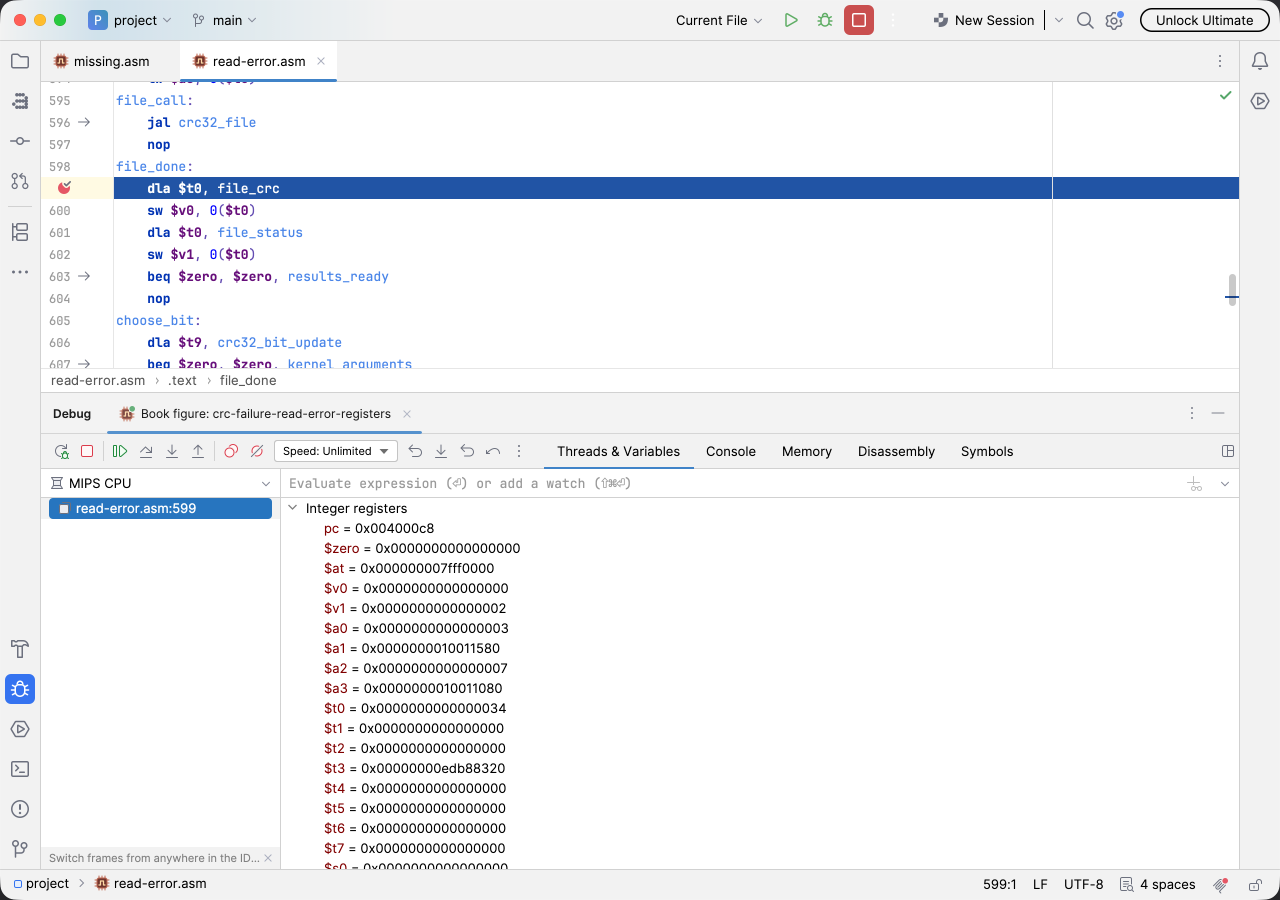
\includegraphics[width=0.54\linewidth,artifact,trim={\MARScrcFailuresourceLeft{} \MARScrcFailuresourceBottom{} \MARScrcFailuresourceRight{} \MARScrcFailuresourceTop{}},clip]{packages/024-crc32/captures/f04/read-error-registers.png}};
    \begin{scope}[shift={(source.south west)},x={($(source.south east)-(source.south west)$)},y={($(source.north west)-(source.south west)$)}]
      \draw[black,line width=0.7pt] (0.215625000,0.080000000) rectangle (0.725000000,0.520000000);
      \node[draw=black,fill=white,circle,inner sep=1.5pt,font=\footnotesize] at ($(0.215625000,0.520000000)+(-3mm,0)$) {1};
    \end{scope}
    \node[anchor=north west,inner sep=0,font=\small\bfseries] (missing-title) at ([yshift=-1mm]source.south west) {Missing path: returned values};
    \node[anchor=north west,inner sep=0] (missing) at ([yshift=-1mm]missing-title.south west) {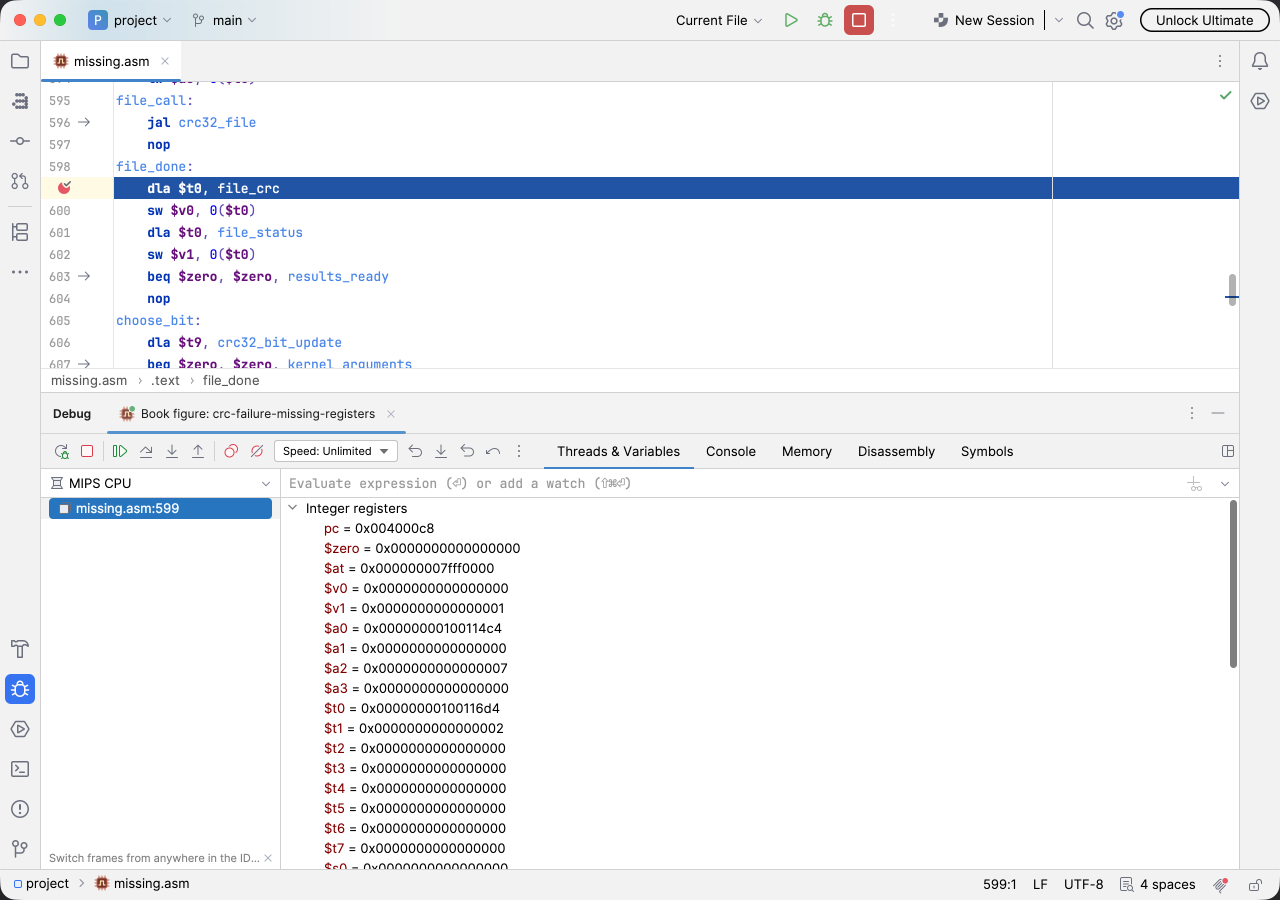
\includegraphics[width=0.44\linewidth,artifact,trim={\MARScrcFailuremissingLeft{} \MARScrcFailuremissingBottom{} \MARScrcFailuremissingRight{} \MARScrcFailuremissingTop{}},clip]{packages/024-crc32/captures/f04/missing-registers.png}};
    \begin{scope}[shift={(missing.south west)},x={($(missing.south east)-(missing.south west)$)},y={($(missing.north west)-(missing.south west)$)}]
      \draw[black,line width=0.7pt] (0.023437500,0.023255814) rectangle (0.761718750,0.953488372);
      \node[draw=black,fill=white,circle,inner sep=1.5pt,font=\footnotesize] at ($(0.023437500,0.953488372)+(-3mm,0)$) {2};
    \end{scope}
    \node[anchor=north west,inner sep=0,font=\small\bfseries] (readerror-title) at (0.54\linewidth,0 |- missing-title.north) {Read error: returned values};
    \node[anchor=north west,inner sep=0] (readerror) at ([yshift=-1mm]readerror-title.south west) {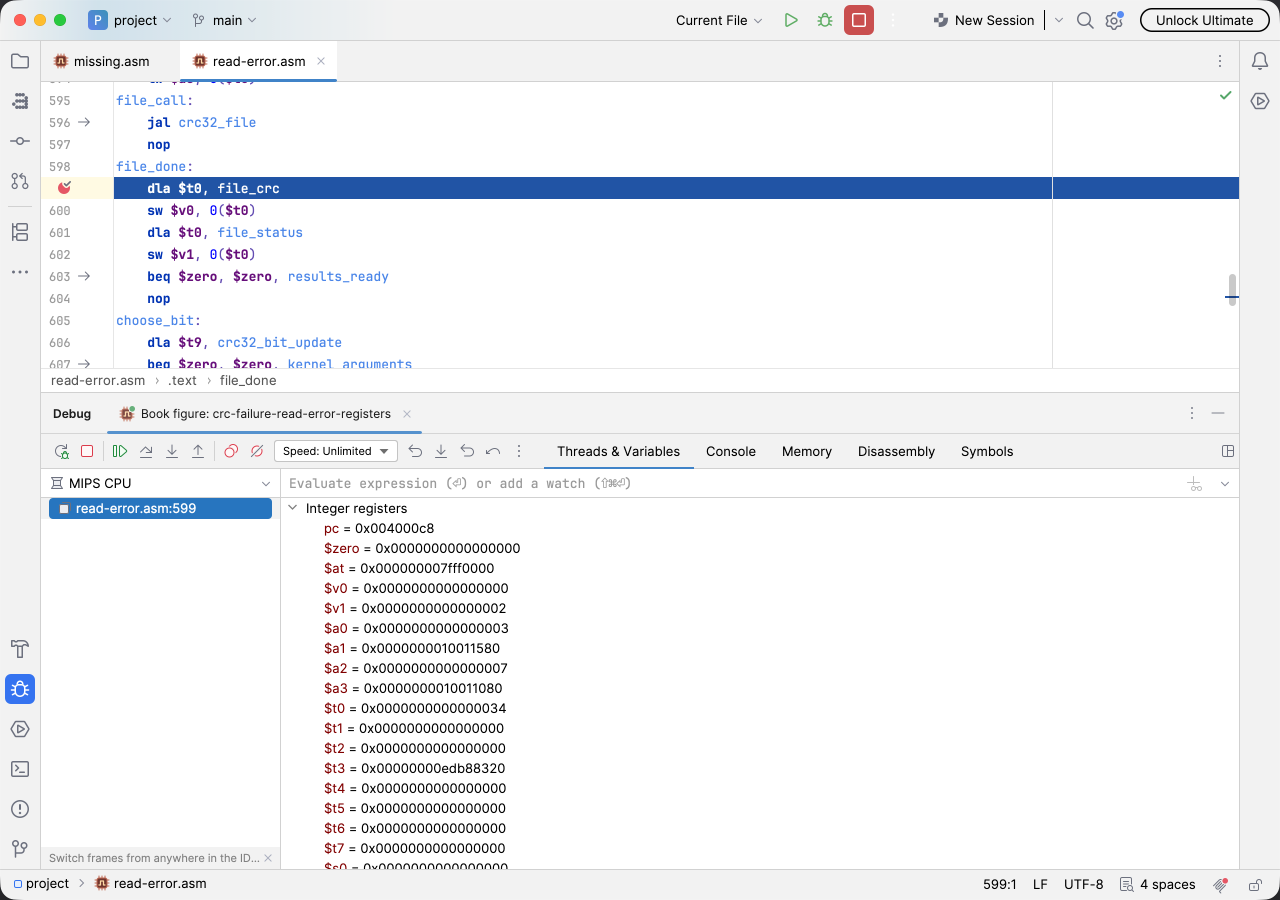
\includegraphics[width=0.44\linewidth,artifact,trim={\MARScrcFailurereaderrorLeft{} \MARScrcFailurereaderrorBottom{} \MARScrcFailurereaderrorRight{} \MARScrcFailurereaderrorTop{}},clip]{packages/024-crc32/captures/f04/read-error-registers.png}};
    \begin{scope}[shift={(readerror.south west)},x={($(readerror.south east)-(readerror.south west)$)},y={($(readerror.north west)-(readerror.south west)$)}]
      \draw[black,line width=0.7pt] (0.023437500,0.023255814) rectangle (0.761718750,0.953488372);
      \node[draw=black,fill=white,circle,inner sep=1.5pt,font=\footnotesize] at ($(0.023437500,0.953488372)+(-3mm,0)$) {3};
    \end{scope}
    \node[anchor=north west,inner sep=0,font=\small\bfseries] (missingscratch-title) at ([yshift=-1mm]missing.south west) {Missing path: unchanged scratch};
    \node[anchor=north west,inner sep=0] (missingscratch) at ([yshift=-1mm]missingscratch-title.south west) {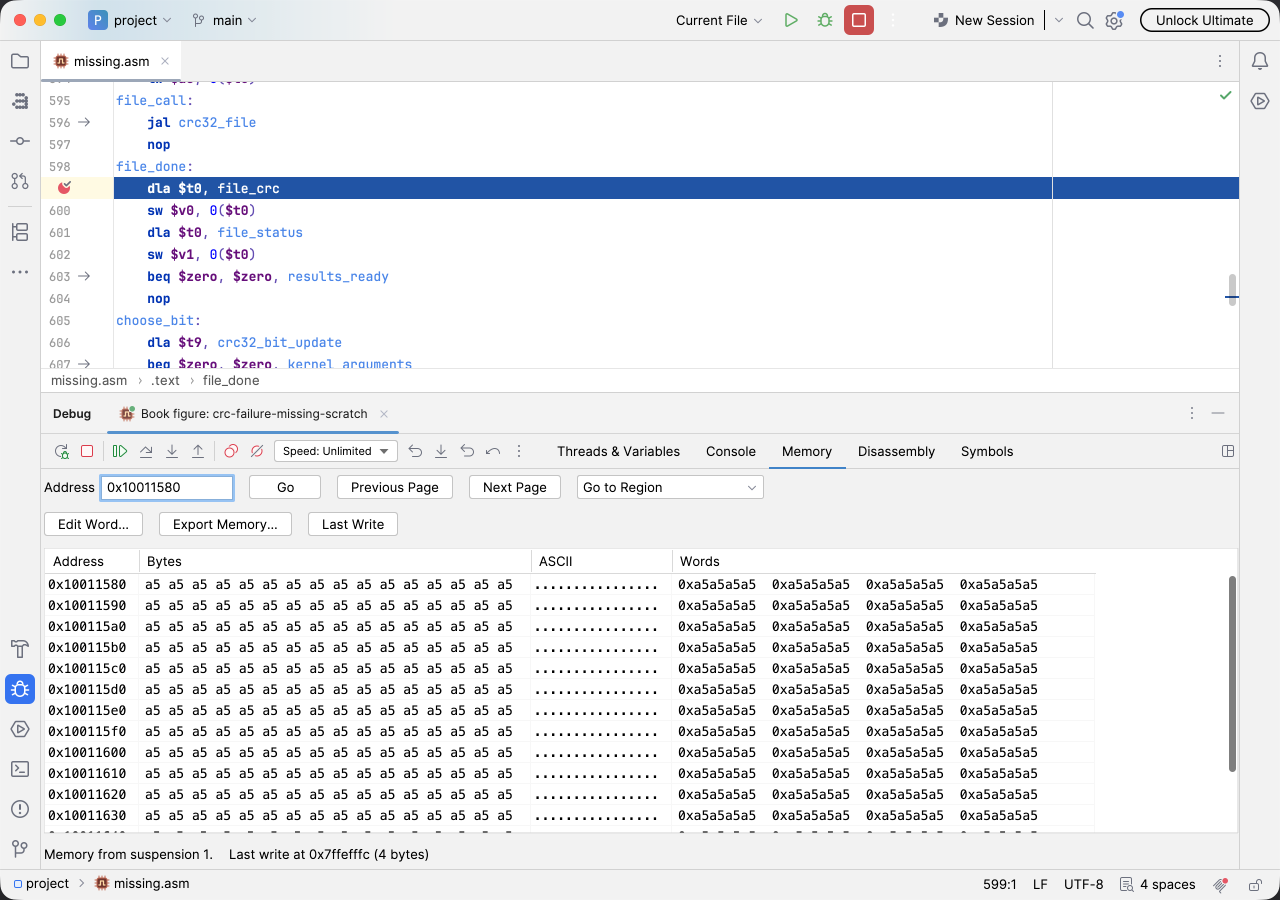
\includegraphics[width=0.84\linewidth,artifact,trim={\MARScrcFailuremissingscratchLeft{} \MARScrcFailuremissingscratchBottom{} \MARScrcFailuremissingscratchRight{} \MARScrcFailuremissingscratchTop{}},clip]{packages/024-crc32/captures/f04/missing-scratch.png}};
    \begin{scope}[shift={(missingscratch.south west)},x={($(missingscratch.south east)-(missingscratch.south west)$)},y={($(missingscratch.north west)-(missingscratch.south west)$)}]
      \draw[black,line width=0.7pt] (0.194672131,0.078431373) rectangle (0.997950820,0.490196078);
      \node[draw=black,fill=white,circle,inner sep=1.5pt,font=\footnotesize] at ($(0,0.490196078)+(-3mm,0)$) {4};
    \end{scope}
    \node[anchor=north west,inner sep=0,font=\small\bfseries] (errorscratch-title) at ([yshift=-1mm]missingscratch.south west) {Read error: overwritten prefix};
    \node[anchor=north west,inner sep=0] (errorscratch) at ([yshift=-1mm]errorscratch-title.south west) {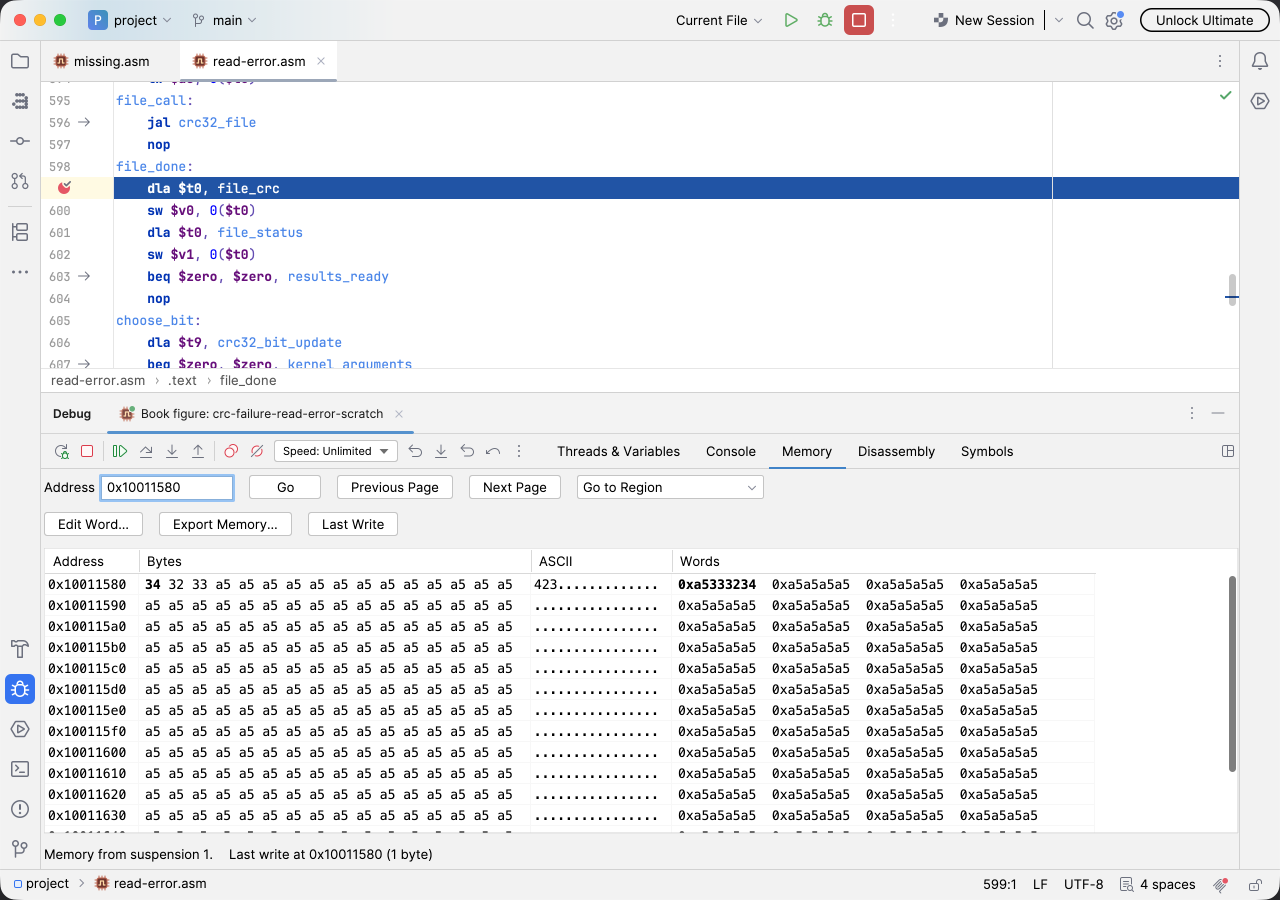
\includegraphics[width=0.84\linewidth,artifact,trim={\MARScrcFailureerrorscratchLeft{} \MARScrcFailureerrorscratchBottom{} \MARScrcFailureerrorscratchRight{} \MARScrcFailureerrorscratchTop{}},clip]{packages/024-crc32/captures/f04/read-error-scratch.png}};
    \begin{scope}[shift={(errorscratch.south west)},x={($(errorscratch.south east)-(errorscratch.south west)$)},y={($(errorscratch.north west)-(errorscratch.south west)$)}]
      \draw[black,line width=0.7pt] (0.194672131,0.078431373) rectangle (0.997950820,0.490196078);
      \node[draw=black,fill=white,circle,inner sep=1.5pt,font=\footnotesize] at ($(0,0.490196078)+(-3mm,0)$) {5};
    \end{scope}
    \node[anchor=north west,inner sep=0,font=\small\bfseries] (control-title) at ([yshift=-1mm]errorscratch.south west) {Caller controls and unpublished results};
    \node[anchor=north west,inner sep=0] (control) at ([yshift=-1mm]control-title.south west) {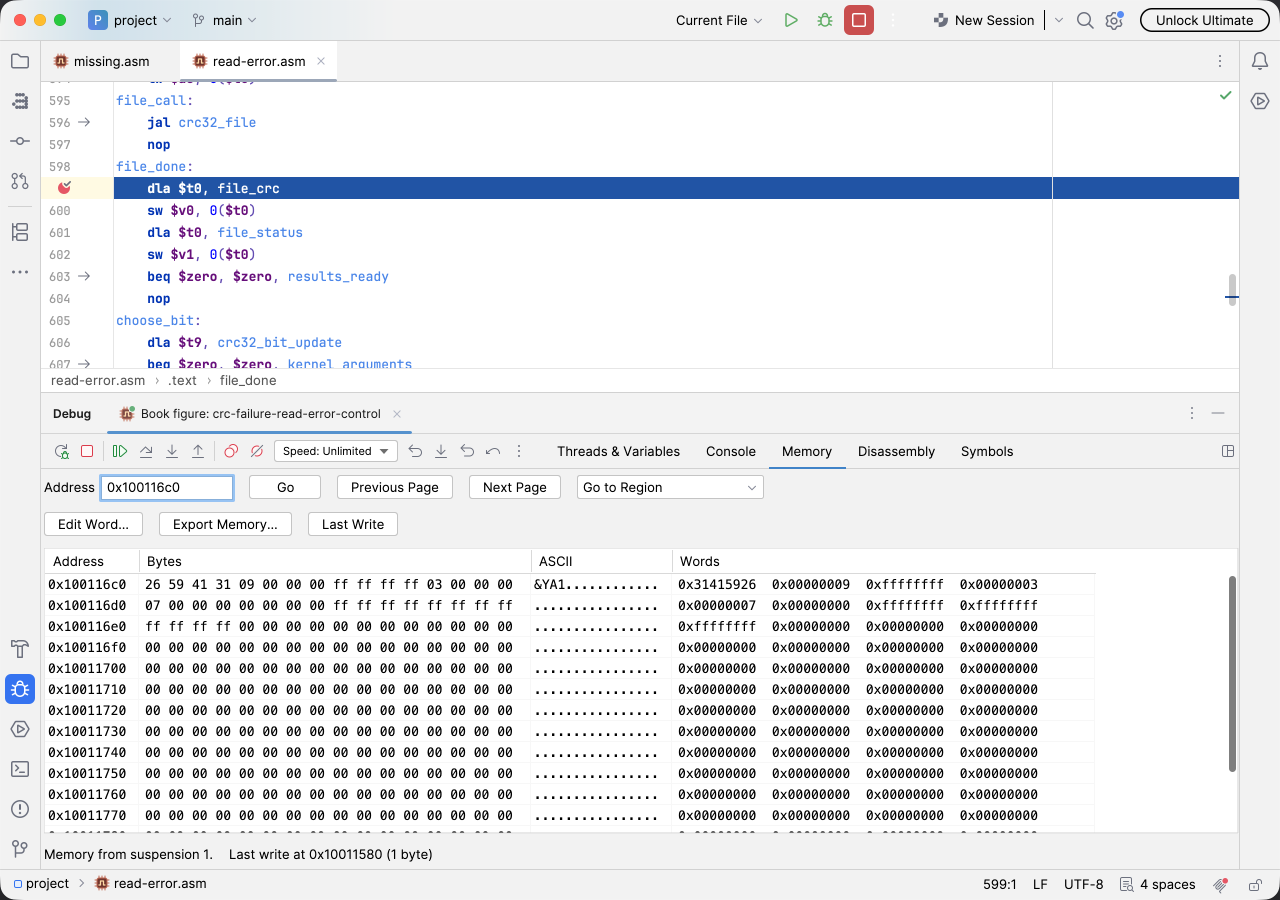
\includegraphics[width=0.84\linewidth,artifact,trim={\MARScrcFailurecontrolLeft{} \MARScrcFailurecontrolBottom{} \MARScrcFailurecontrolRight{} \MARScrcFailurecontrolTop{}},clip]{packages/024-crc32/captures/f04/read-error-control.png}};
    \begin{scope}[shift={(control.south west)},x={($(control.south east)-(control.south west)$)},y={($(control.north west)-(control.south west)$)}]
      \draw[black,line width=0.7pt] (0.194672131,0.055555556) rectangle (0.997950820,0.638888889);
      \node[draw=black,fill=white,circle,inner sep=1.5pt,font=\footnotesize] at ($(0,0.638888889)+(-3mm,0)$) {6};
    \end{scope}
  \end{tikzpicture}
  \par\smallskip
  \begin{minipage}{\linewidth}
    \small
    \begin{enumerate}
      \setlength{\itemsep}{0pt}
            \setlength{\parsep}{0pt}
      \item The stop at \texttt{file\_done} precedes the caller stores. These are explicit in-memory fixtures supplied by the authoring plugin: a missing path and a read failure after four bytes. The simulated function instructions are unchanged.
      \item The missing path returns \texttt{v0 = 0} and \texttt{v1 = 1}. Its open returns $-1$, so no descriptor was acquired and there is none for the guest to close.
      \item The read-error path returns \texttt{v0 = 0} and \texttt{v1 = 2}. Its operation receipt records open, reads of three bytes and one byte, a failed read, then guest close. Closure is checked from this history, not inferred from register values.
      \item Missing-path scratch remains \texttt{a5}. The full memory history confirms that the function did not write it.
      \item Read-error scratch begins \texttt{34 32 33}. The one-byte second read replaces only the initial \texttt{31}; \texttt{32 33} remain from the first read. The function consumed four bytes in total, not three from this final buffer view.
      \item The controls retain capacity seven and bit method zero. The displayed \texttt{raw\_result} and \texttt{file\_crc} words are still $-1$. The fixture limits positive reads to three bytes and fails at four consumed bytes. A nonzero status makes \texttt{v0} unusable as a checksum; the caller publishes the return values afterward.
    \end{enumerate}
  \end{minipage}
  \caption{Distinct file failures return a status and no public checksum.}
  \label{capture:024-crc32-f04}
  \label{crc-f04}
\end{figure}
\par
